\section{A.R.E.S.}

\subsection{Vehicle Architecture}

The AURORA Rocket and Experimental Systems (\ares{}) vehicle is a 10.5-foot-tall, 6-inch-diameter high-power research rocket currently being designed and manufactured at the University of Hartford. The vehicle serves as the primary flight platform for the capstone and carries the \deimos{} telemetry system, \phobos{} experimental RF payload, \comet{} recovery flight computer, and associated recovery and support hardware.

The airframe is being constructed primarily from fiberglass components to provide the strength and durability required for repeated high-power flight operations. A modular architecture is being used so that the nose cone, avionics, experimental payload, recovery, and propulsion sections can be independently assembled, inspected, serviced, and tested before final integration.

Structural interfaces, internal mounting systems, recovery attachment points, and fin connections are being designed around the aerodynamic and inertial loads expected during flight. Wherever practical, components are being designed so that individual subsystems can be removed, modified, and reinstalled without requiring major reconstruction of the vehicle.

\subsection{Aerodynamic and Structural Analysis}

Mechanical design and structural verification of \ares{} will be led by Liam Gordon. The design process is intended to ensure that the final vehicle satisfies real-world aerodynamic, structural, and mechanical strength requirements prior to fabrication and flight.

Computational fluid dynamics (CFD) will be used where appropriate to investigate aerodynamic behavior and loading. Finite element analysis (FEA) using ANSYS and Onshape will be used to evaluate structural stresses, deflection, and load paths through critical components. Particular attention will be placed on highly loaded regions including fin attachment interfaces, motor-support structure, recovery attachment hardware, and joints between major airframe sections.

Results from these analyses will be used to iteratively refine component geometry, material selection, and manufacturing methods before flight hardware is finalized.

OpenRocket is also being used throughout the design process to evaluate the predicted flight behavior of the vehicle. OpenRocket calculates parameters including center of gravity, center of pressure, stability, acceleration, velocity, and predicted altitude and allows these properties to be evaluated as the vehicle configuration changes \cite{niskanen,openrocket}. Vehicle mass, payload placement, propulsion selection, aerodynamic geometry, and measured component properties will be incorporated into the model as the physical vehicle is completed.

The development of \ares{} builds upon experience obtained through previous AURORA high-power rocket projects, including Nicholas Krupa's successful Level 2 certification flight and subsequent high-power launches. Data and practical experience from these vehicles are being used to inform stability, recovery, avionics integration, manufacturing, and launch-operation decisions as the team transitions toward a substantially larger vehicle. The Level 2 certification vehicle that contributed to this design experience is shown in Fig.~\ref{fig:l2_rocket}.

\begin{figure}[htbp]
    \centering
    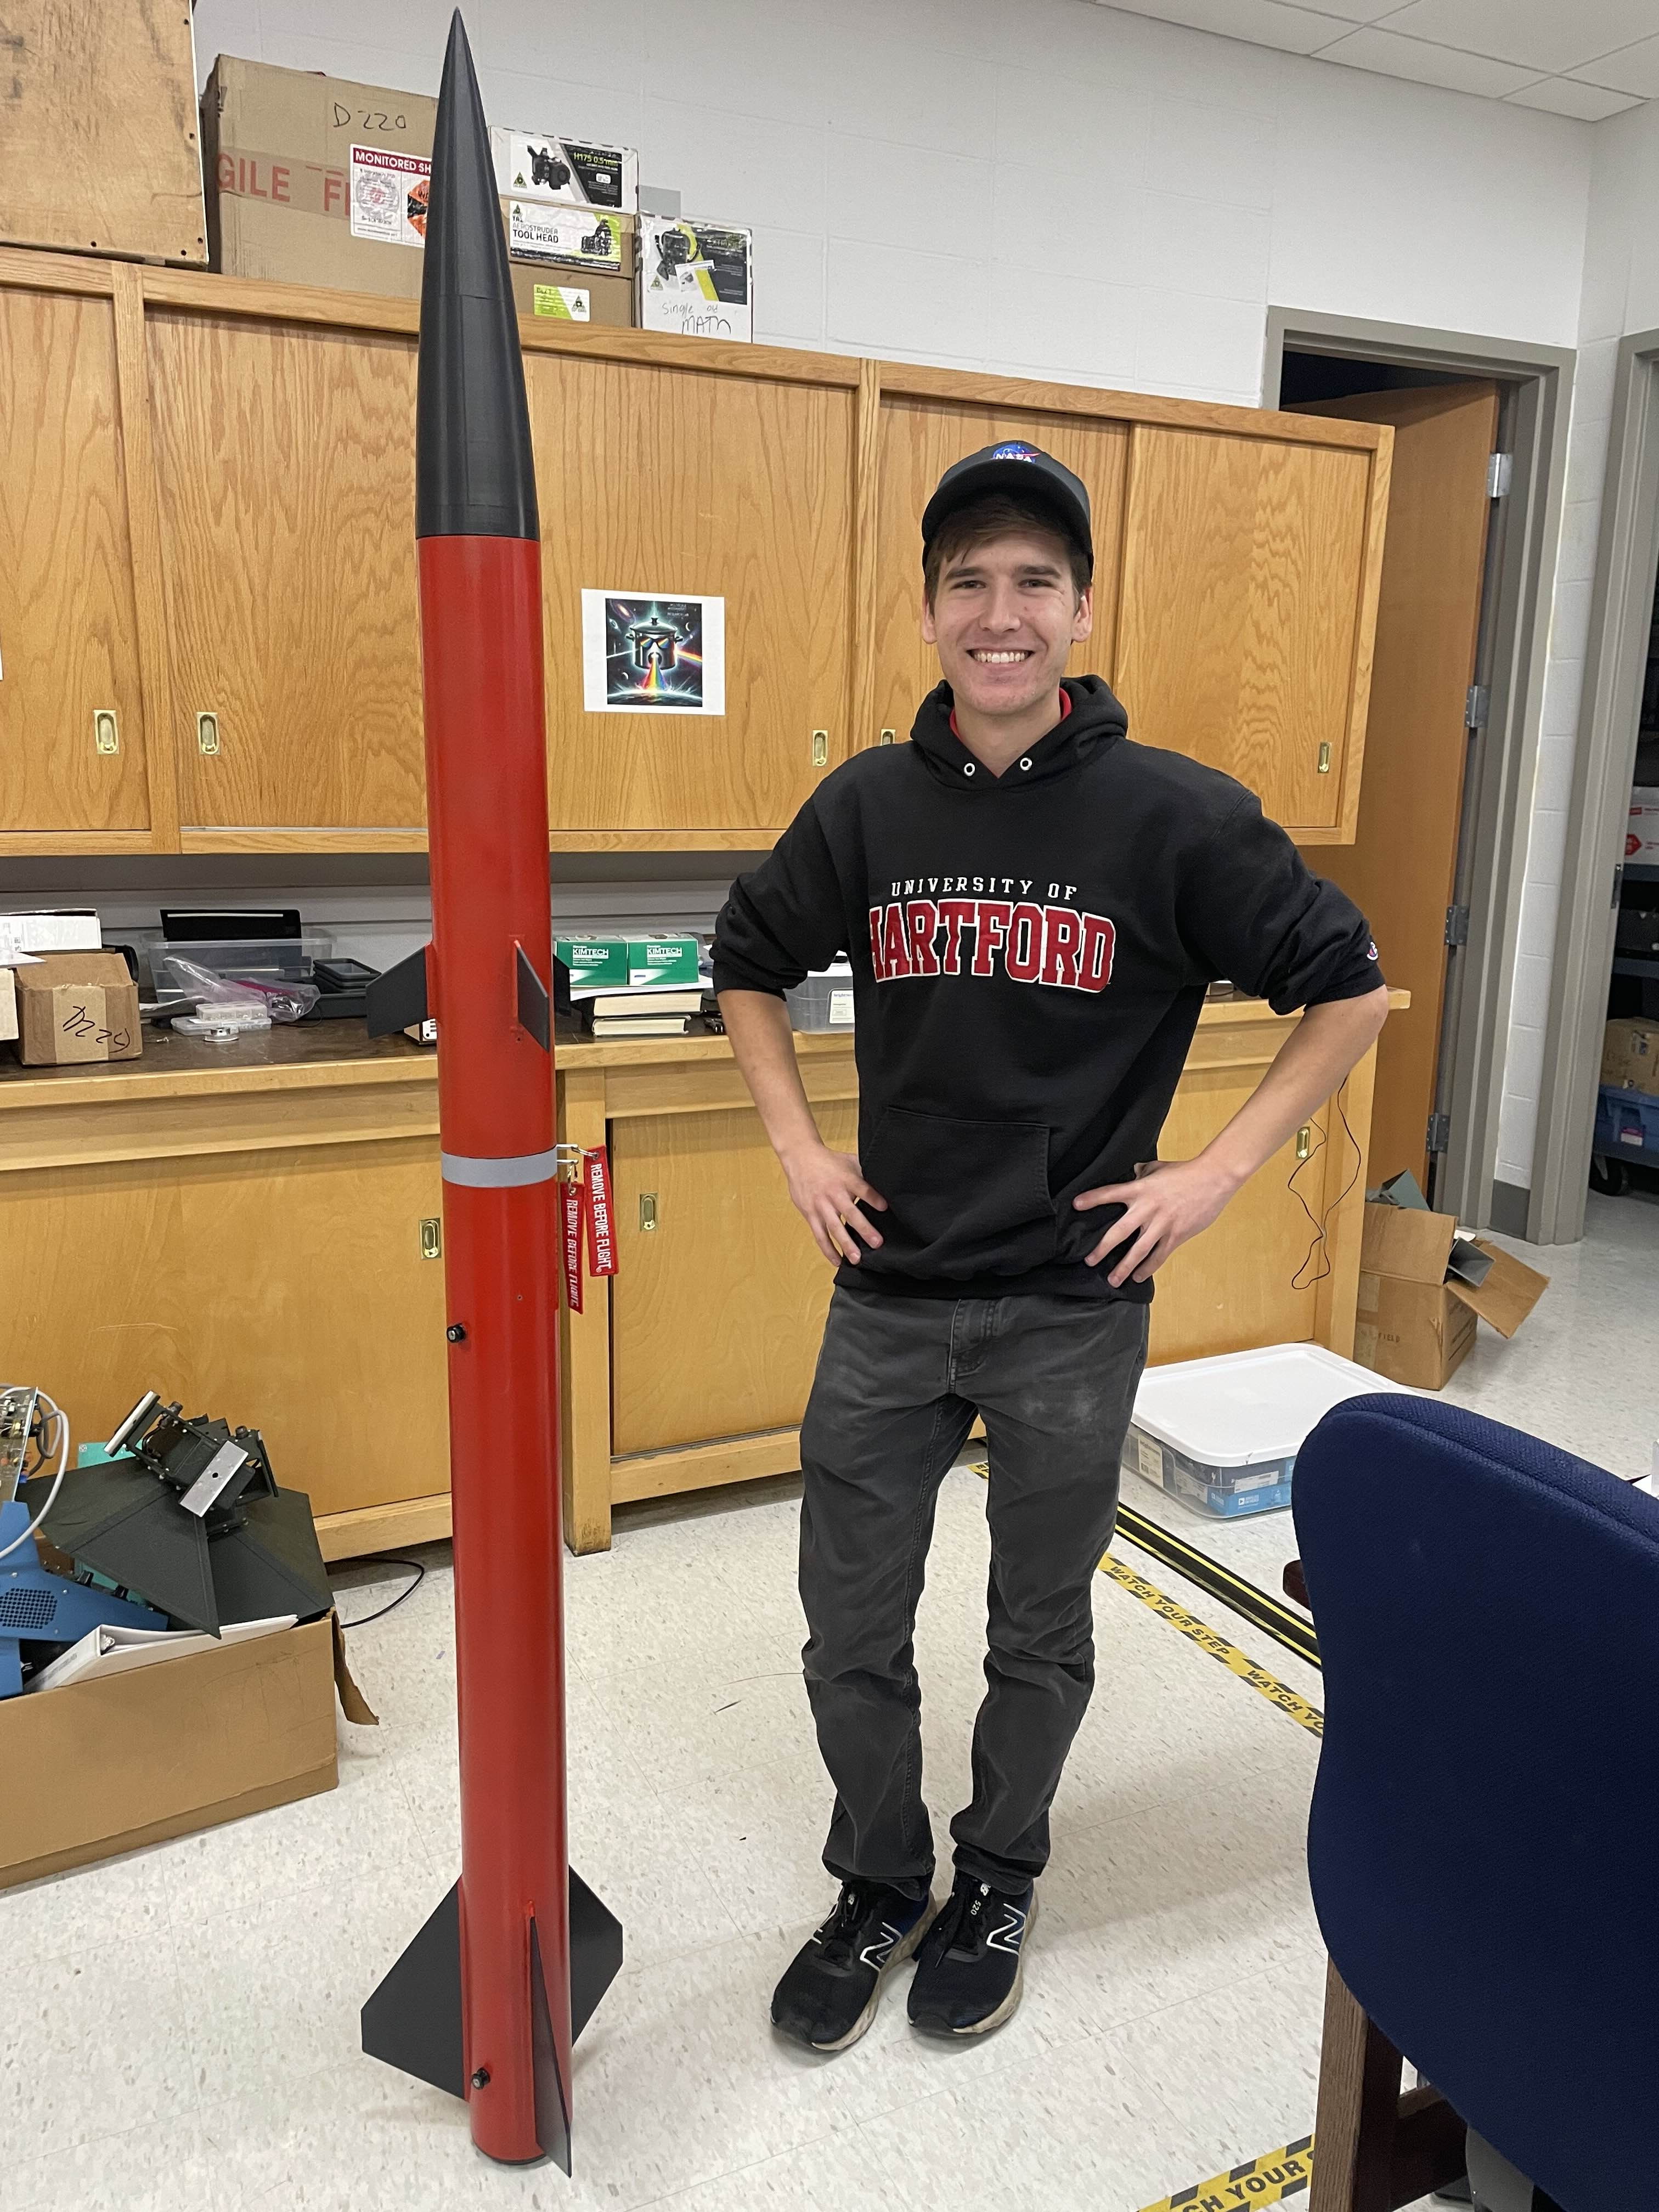
\includegraphics[width=\columnwidth]{L2Rocket.jpg}
    \caption{Nicholas Krupa with the AURORA high-power rocket used for his successful National Association of Rocketry Level 2 certification flight. The vehicle provided prior flight experience in stability, recovery, avionics integration, and high-power launch operations that is being applied to the development of \ares{}.}
    \label{fig:l2_rocket}
\end{figure}

\subsection{Propulsion and Recovery}

The propulsion system will be selected to provide sufficient performance for the fully integrated vehicle while maintaining acceleration, velocity, stability, and structural loading within acceptable design limits. Motor selection will therefore be evaluated alongside final vehicle mass, aerodynamic performance, expected altitude, and payload requirements.

The propulsion section will be designed so that certified commercial motor hardware can be installed and inspected independently from the remaining vehicle systems. Final motor selection and launch operations will remain within the certification, launch-site, and safety requirements applicable to each flight.

A dual-deployment recovery architecture will be used to return the vehicle following flight. Separate drogue and main parachute events will control descent while limiting vehicle drift. Recovery events will be commanded by the \comet{} flight computer, while the \ares{} structure will contain the parachutes, harnesses, attachment hardware, deployment compartments, and associated recovery hardware.

Recovery-system ground testing will be completed prior to flight to verify reliable compartment separation, parachute extraction, and integrated system operation. Final launch and recovery operations will be conducted through an established high-power rocketry organization and in accordance with applicable launch-site, FAA, and high-power rocketry safety requirements \cite{narsafety}.

\subsection{Manufacturing and Integration}

Construction of \ares{} will occur in parallel with development of the electrical and experimental systems. This approach allows mechanical, electrical, and RF interfaces to be evaluated throughout the project rather than only during final assembly.

Fiberglass fabrication, structural bonding, machining, additive manufacturing, avionics mounting, wiring, and final vehicle assembly will form a significant portion of the capstone effort. Major interfaces will be inspected and tested before full-system integration.

Prior to flight, the vehicle will undergo simulation review, structural analysis, subsystem testing, recovery testing, integration testing, and flight-readiness review. Through this process, \ares{} is intended to demonstrate the successful integration of aerodynamic design, structural engineering, propulsion, recovery, avionics, telemetry, and experimental RF systems into a single high-power research platform.

At the time of writing, external industry sponsorship for the \ares{} vehicle is being discussed with Ensign-Bickford Aerospace \& Defense (EBAD). Prospective support would contribute directly to vehicle materials, propulsion, structural hardware, manufacturing, and ground and flight testing.

% =========================================================
\section{P.H.O.B.O.S.}
\subsection{Introduction}
Development of the \phobos{} experimental RF payload is supported through a NASA Connecticut Space Grant Consortium Undergraduate Research Grant awarded to Kyle Eckert during the Spring 2026 award cycle \cite{ctsgc2026}. The research is intended to investigate the performance of directional RF communication and beam-steering technologies when transferred from a laboratory environment to a moving rocket platform.

The original grant proposal was developed around a competition-based rocket mission and a \SI{5}{\giga\hertz} experimental implementation. Following revision of the overall vehicle mission, the underlying research objective has been retained while the flight platform and final RF implementation are being reevaluated for integration with \ares{}.

\subsection{Phased-Array Antenna}

The primary objective of the \phobos{} phased-array antenna system is to electronically alter the direction of RF transmission based on the relative geometry between the rocket and a receiving ground station. In a phased array, controlled phase relationships between multiple radiating elements cause constructive and destructive interference that can shift the direction of the primary radiation pattern without mechanically rotating the antenna \cite{balanis}. A conceptual example of this beam-steering behavior is shown in Fig.~\ref{fig:phobos_beam_steering}.

\begin{figure}[htbp]
    \centering
    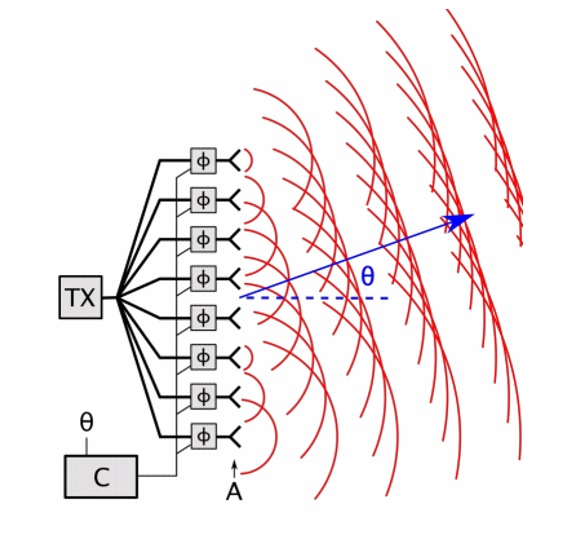
\includegraphics[width=0.95\columnwidth]{PAA/PAA_Ex.png}
    \caption{Conceptual illustration of phased-array beam steering. Controlled phase offsets between antenna elements alter the direction of constructive interference, allowing the main radiation lobe to be electronically steered without mechanically rotating the antenna.}
    \label{fig:phobos_beam_steering}
\end{figure}
% If PAA_Ex.png was obtained from an external source, add the appropriate citation to the caption above.

For the current design, operation near \SI{2.4}{\giga\hertz} is being investigated as a strong candidate because it provides a practical compromise between antenna dimensions, available RF hardware, communication bandwidth, and vehicle packaging constraints. The final operating frequency will be selected following additional antenna design, link-budget analysis, and subsystem testing.

Because the system is an intentional RF radiator, regulatory compliance will be considered throughout development. For digitally modulated systems operating under FCC Part 15, 47~CFR~\S15.247 includes operation within the 2400--2483.5~MHz band and establishes requirements involving occupied bandwidth, conducted transmitter power, spectral density, and antenna gain \cite{fcc247}. Therefore, the final transmitter architecture, output power, modulation method, antenna gain, and array configuration will be evaluated against the regulations applicable to the completed system rather than assuming a single universal unlicensed power limit.

The array must also operate within the geometric constraints of the 6-inch-diameter vehicle. Antenna dimensions scale with wavelength, producing a direct trade between operating frequency, available array aperture, element spacing, and achievable radiation characteristics. These constraints will be evaluated alongside communication range and link performance before the final array geometry is selected.

The current \phobos{} architecture is progressing toward a distributed control and RF implementation consisting of a control board and an antenna board, as summarized in Fig.~\ref{fig:phobos_block_diagram}. The control board has entered the schematic design stage and is intended to contain the primary transceiver and microcontroller. This subsystem will process flight and communication data, control the RF system, and generate the transmitted signal. The resulting RF signal will then be routed to the antenna board, where phase adjustment and any required amplification will occur before the signal is applied to the patch antenna array.

\begin{figure}[htbp]
    \centering
    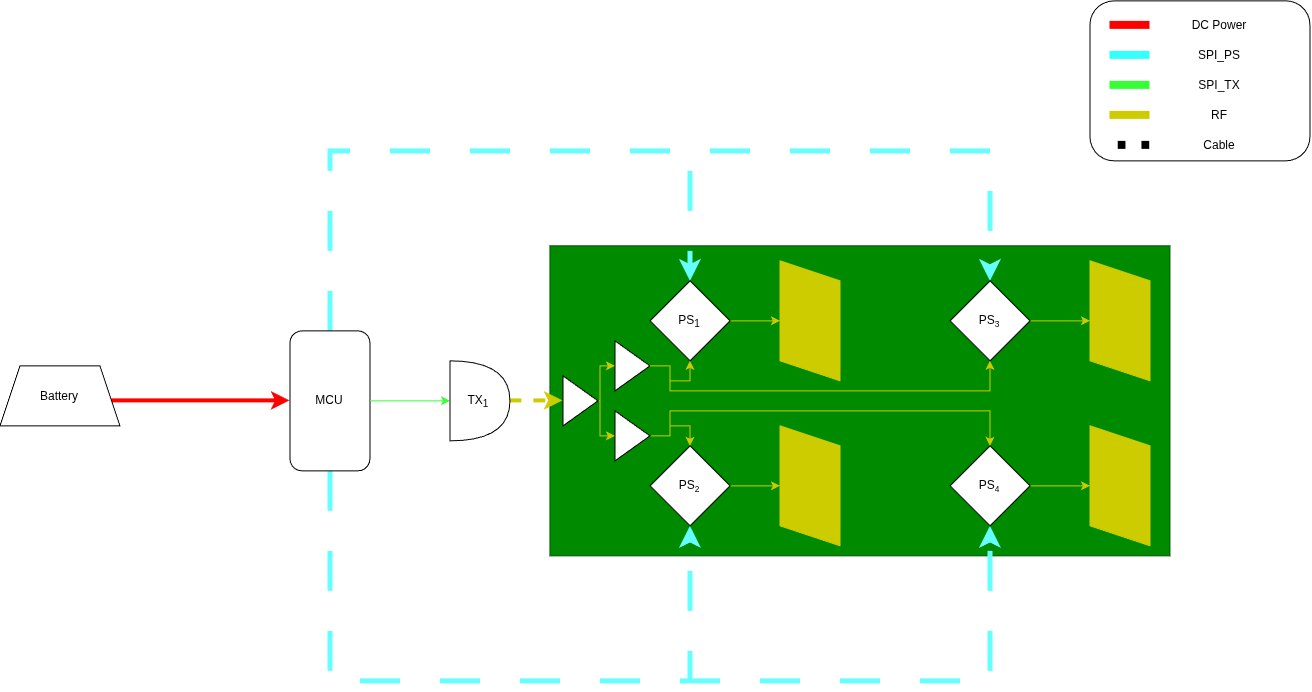
\includegraphics[width=\columnwidth]{PHOBOS/Images/PAA_Block_Diagram.png}
    \caption{Functional block diagram of the proposed \phobos{} architecture. Control and communication functions are separated from the antenna-board RF front end so that signal generation, phase control, amplification, and antenna performance can be developed and tested as distinct subsystems.}
    \label{fig:phobos_block_diagram}
\end{figure}


The control electronics are being developed around a dedicated PCB so that processing, communication, and RF-control functions can be integrated into a compact flight package. The current control-board design is shown in Fig.~\ref{fig:phobos_control_board}, while an example of the associated schematic development is shown in Fig.~\ref{fig:phobos_schematic}.

\begin{figure}[htbp]
    \centering
    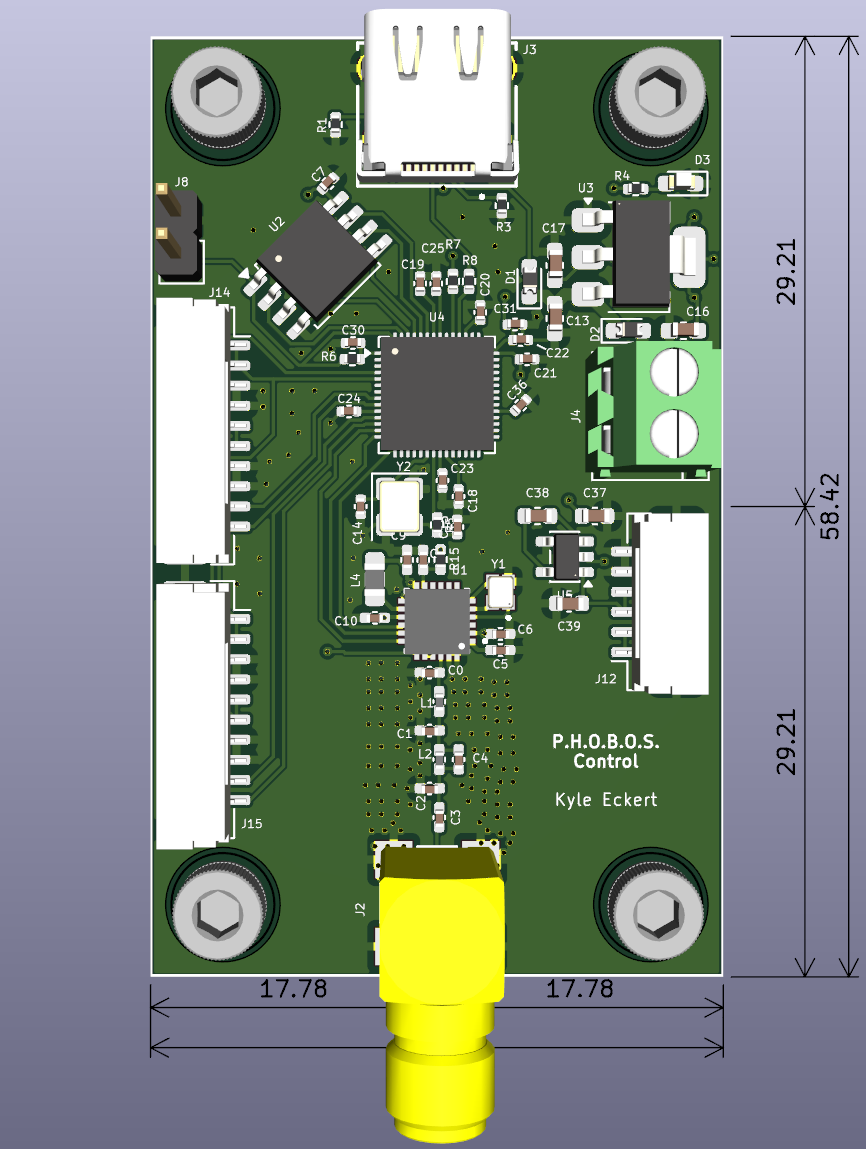
\includegraphics[width=\columnwidth]{Documentation/ARES/PAA/PHOBOS_Control_Board.png}
    \caption{Current \phobos{} control-board design. The board is being developed to integrate the primary microcontroller, transceiver, support electronics, and interfaces required to command the phased-array RF subsystem during flight.}
    \label{fig:phobos_control_board}
\end{figure}

The RF processing architecture on the antenna board is currently in the planning stage. This subsystem is expected to incorporate digitally-controlled phase-shifting devices, RF amplification as required by the link budget, and the individual patch-antenna elements comprising the phased array.
Separating the control and antenna functions into dedicated boards provides flexibility during development and allows the RF front end to be evaluated independently from the primary control electronics.

\begin{figure}[htbp]
    \centering
    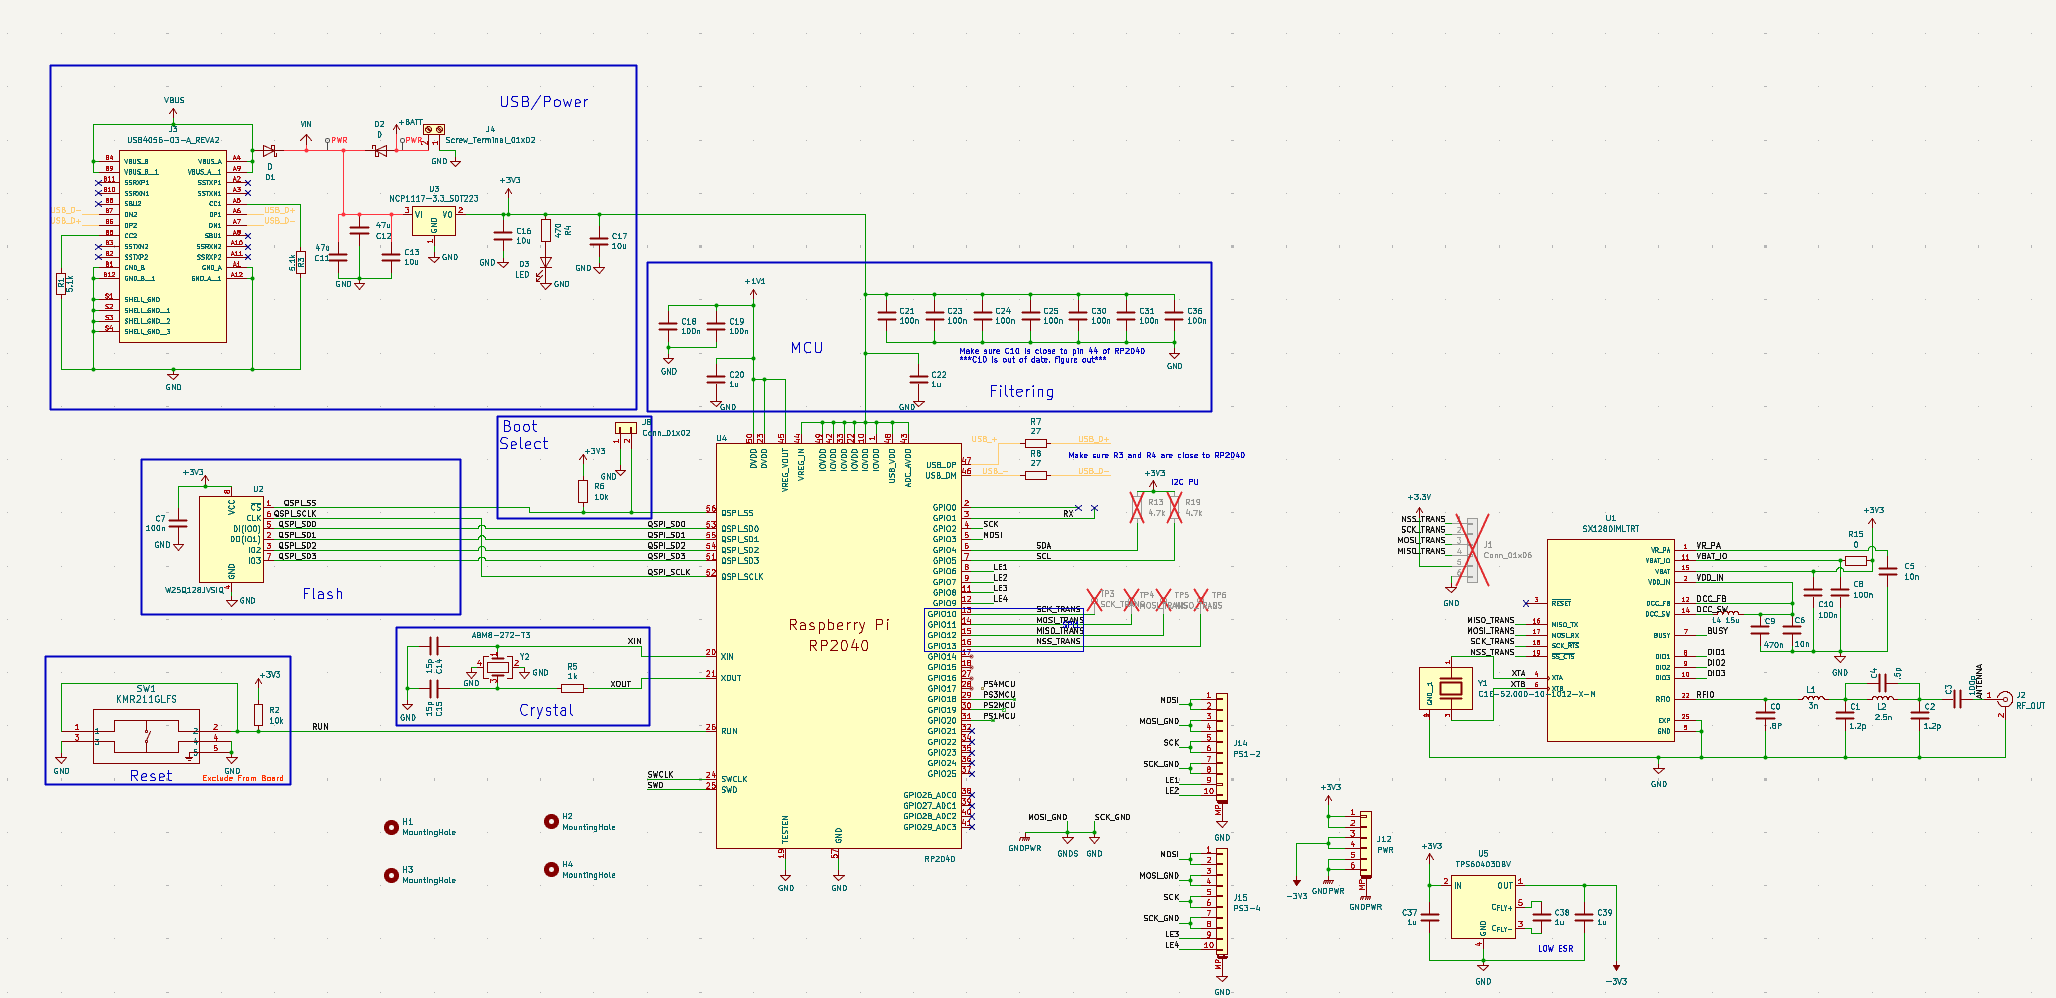
\includegraphics[width=\columnwidth]{Documentation/ARES/PAA/PHOBOS_Control_Schematic.png}
    \caption{The current \phobos{} control-electronics schematic. Schematic development is being used to define the electrical interfaces, signal paths, and support circuitry required before PCB layout and hardware validation.}
    \label{fig:phobos_schematic}
\end{figure}

The completed \phobos{} system is intended to transmit experimental flight data while evaluating whether electronically controlled directional communication can remain useful on a translating and rotating sounding rocket.

% =========================================================
\section{C.O.M.E.T.}

The Compact Onboard Management for Ejection Timing (\comet{}) module is a custom dual-deployment flight computer responsible for controlling the recovery events of the \ares{} vehicle. The system uses onboard barometric and inertial sensing to identify critical portions of the flight and independently control the drogue and main recovery deployment channels.

\comet{} is currently entering its third major hardware revision. Earlier versions have been used to evaluate the sensing, flight-detection, data-logging, and deployment architecture, with the second-generation system undergoing high-power flight testing. Lessons obtained from these tests are being incorporated into the current hardware design, shown in Fig.~\ref{fig:comet_board}.

\begin{figure}[htbp]
    \centering
    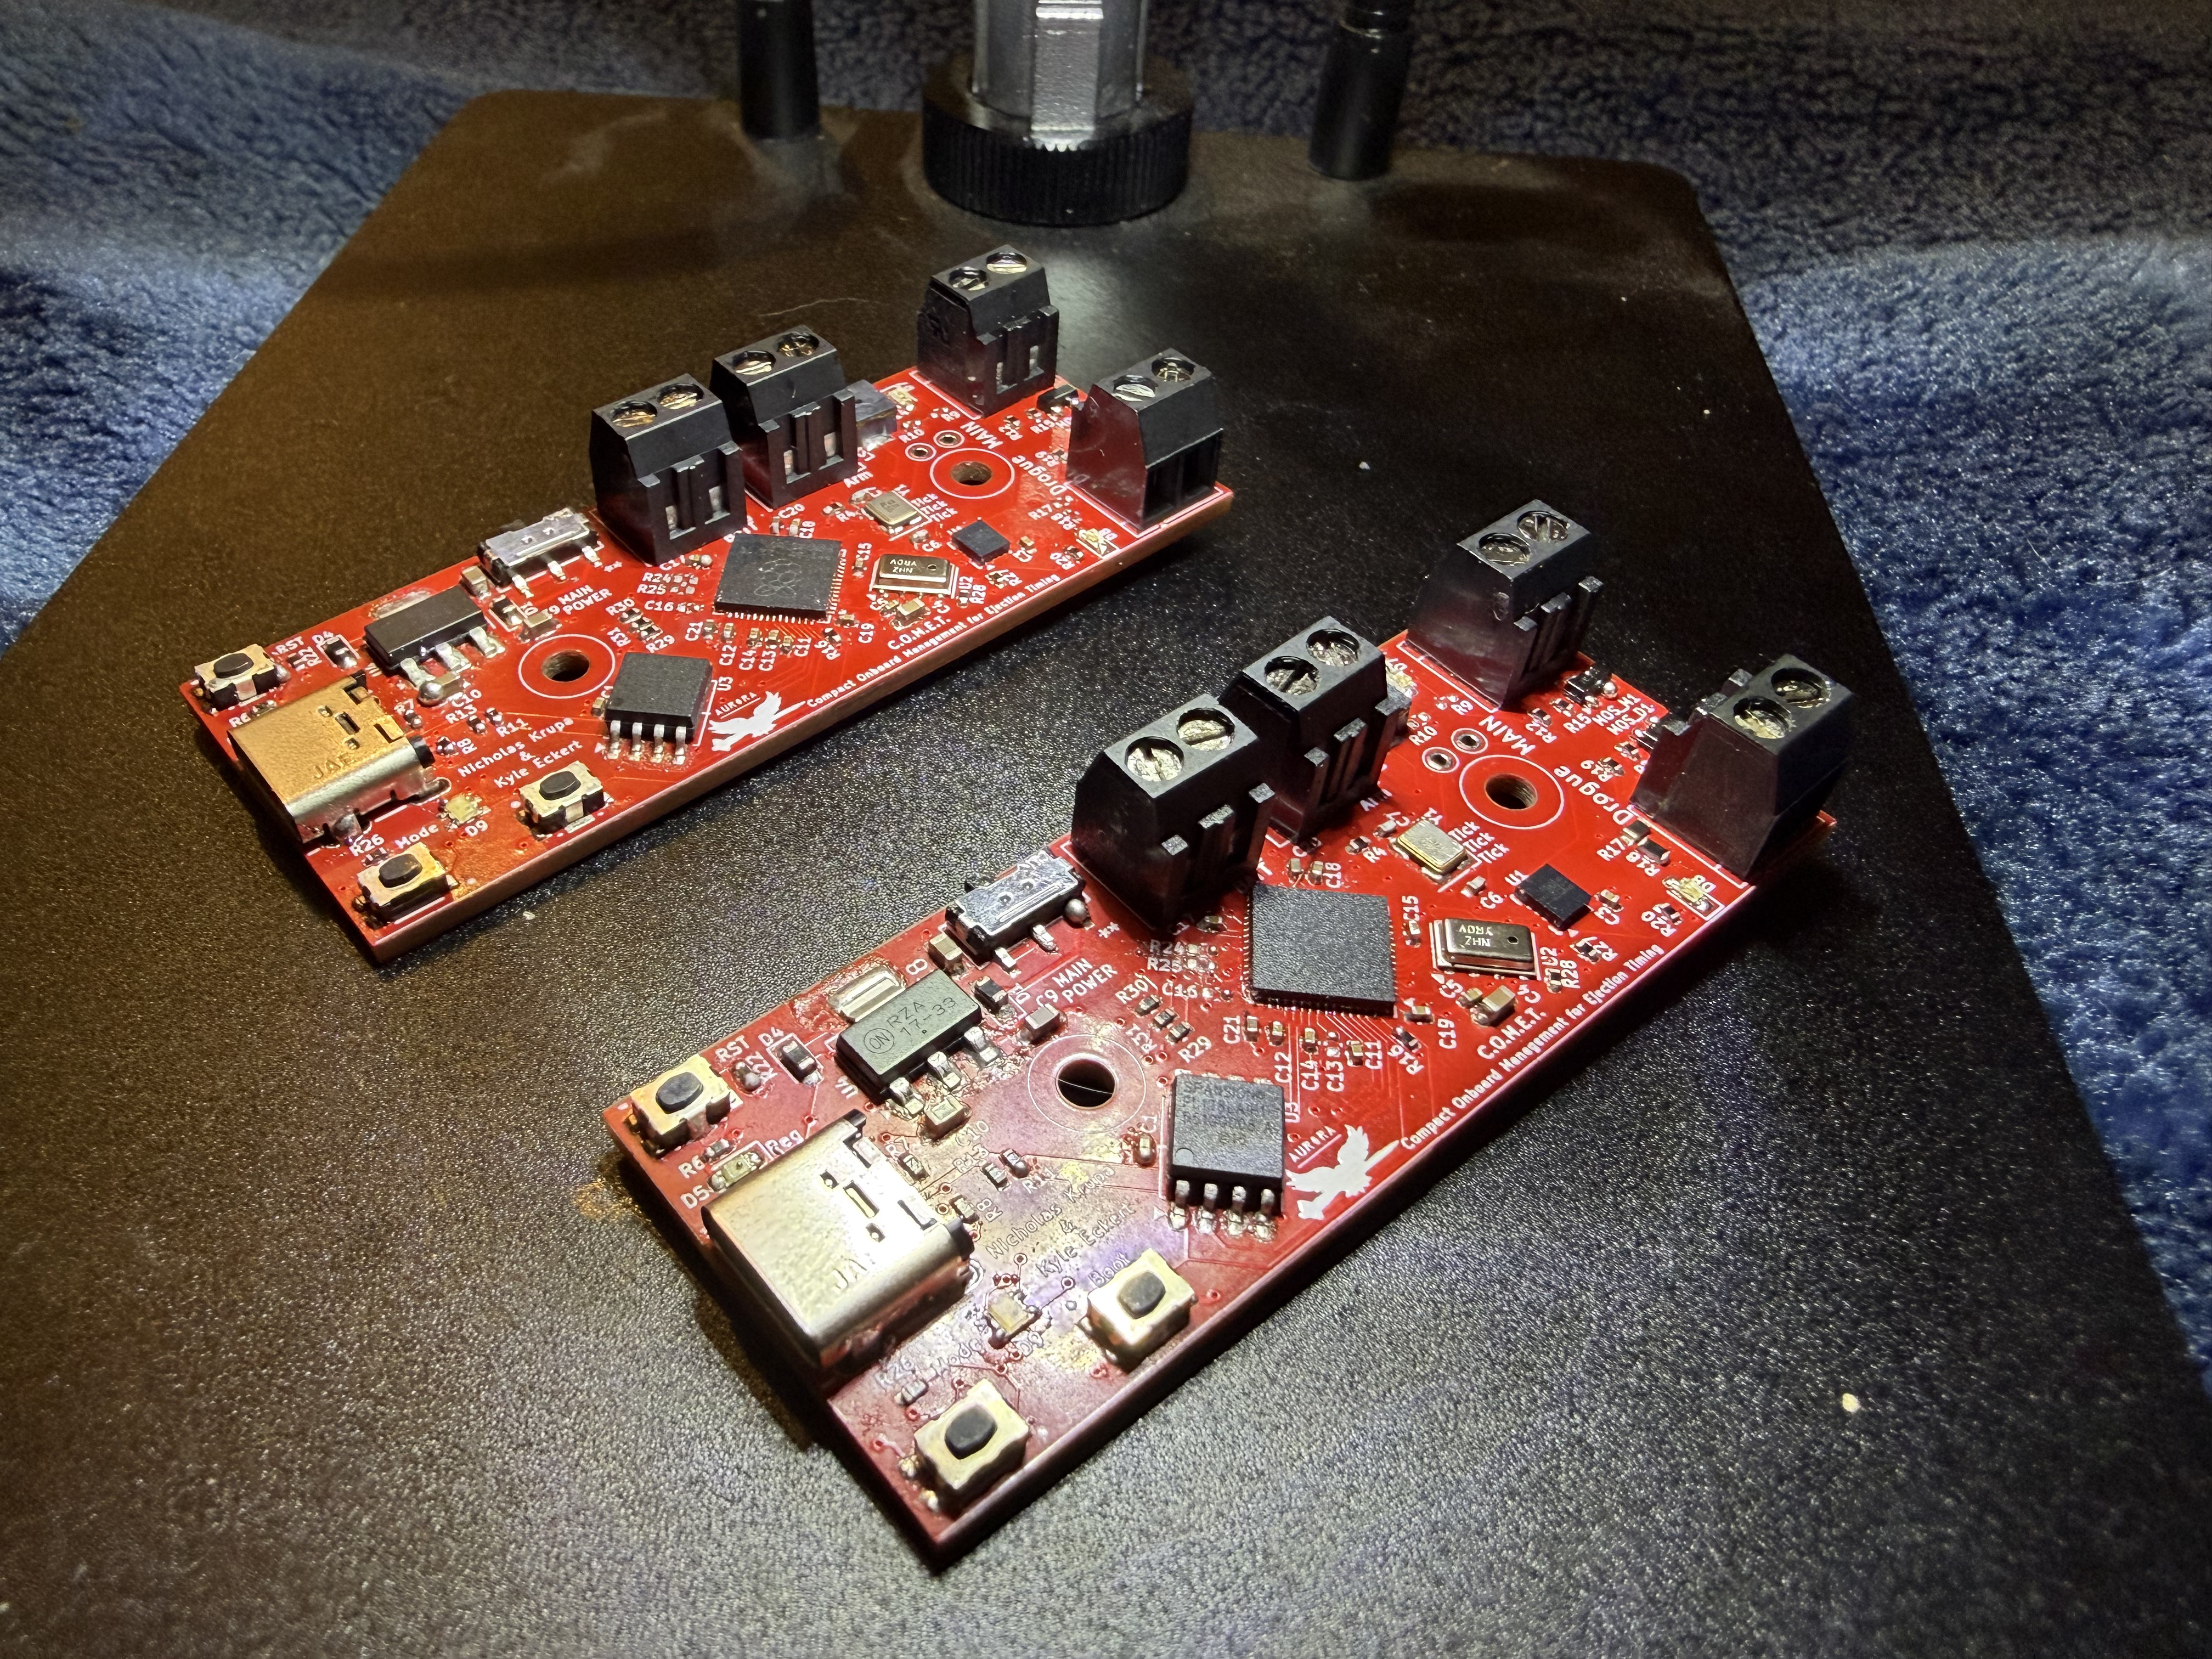
\includegraphics[width=\columnwidth]{COMETBoard.jpg}
    \caption{Current revision of the \comet{} dual-deployment flight computer board. The circuit integrates barometric and inertial sensing, recovery-channel control, power management, continuity monitoring, onboard data logging, and vehicle interfaces onto a compact flight platform.}
    \label{fig:comet_board}
\end{figure}

The flight computer is being developed as a dedicated PCB rather than relying on a collection of independent development boards. The system incorporates onboard sensing, power management, recovery-channel control, continuity monitoring, data logging, user feedback, and interfaces required for vehicle integration.

The flight software is intended to distinguish normal flight conditions from events such as launch, ascent, apogee, and descent while reducing the possibility of an incorrect recovery command caused by transient sensor measurements. Recorded flight data will also allow the operation of the system to be evaluated after each test flight.

Because \comet{} performs a flight-critical function, qualification will emphasize repeatable ground testing and incremental flight validation prior to use as the primary recovery controller for \ares{}. Testing will include sensor verification, electrical load testing, deployment-system testing, data review, and complete integrated recovery testing.

The objective of \comet{} is not only to provide recovery control for the current vehicle, but also to establish a compact student-developed flight-computer architecture that can be reused and improved through future AURORA high-power rocket projects.

% =========================================================
\section{D.E.I.M.O.S.}

The Data Emitting \& Insight Module Orientation System (\deimos{}) is the nose-cone avionics and telemetry subsystem of the \ares{} rocket. The system will contain the sixth generation of the AURORA Insight Module, which has been continuously developed through multiple student engineering projects and high-power rocket flights.

The original Insight Module was developed during the team's freshman year as an engineering expo project and was later expanded during the sophomore year into a more capable telemetry platform. Earlier systems measured parameters including altitude, acceleration, orientation, angular velocity, and position while transmitting flight data to a ground station. The project was recognized as a top engineering expo project and established the technical foundation for the current system. Members of the AURORA team presenting an early generation of the Insight Module are shown in Fig.~\ref{fig:sophomore_expo}.

\begin{figure}[htbp]
    \centering
    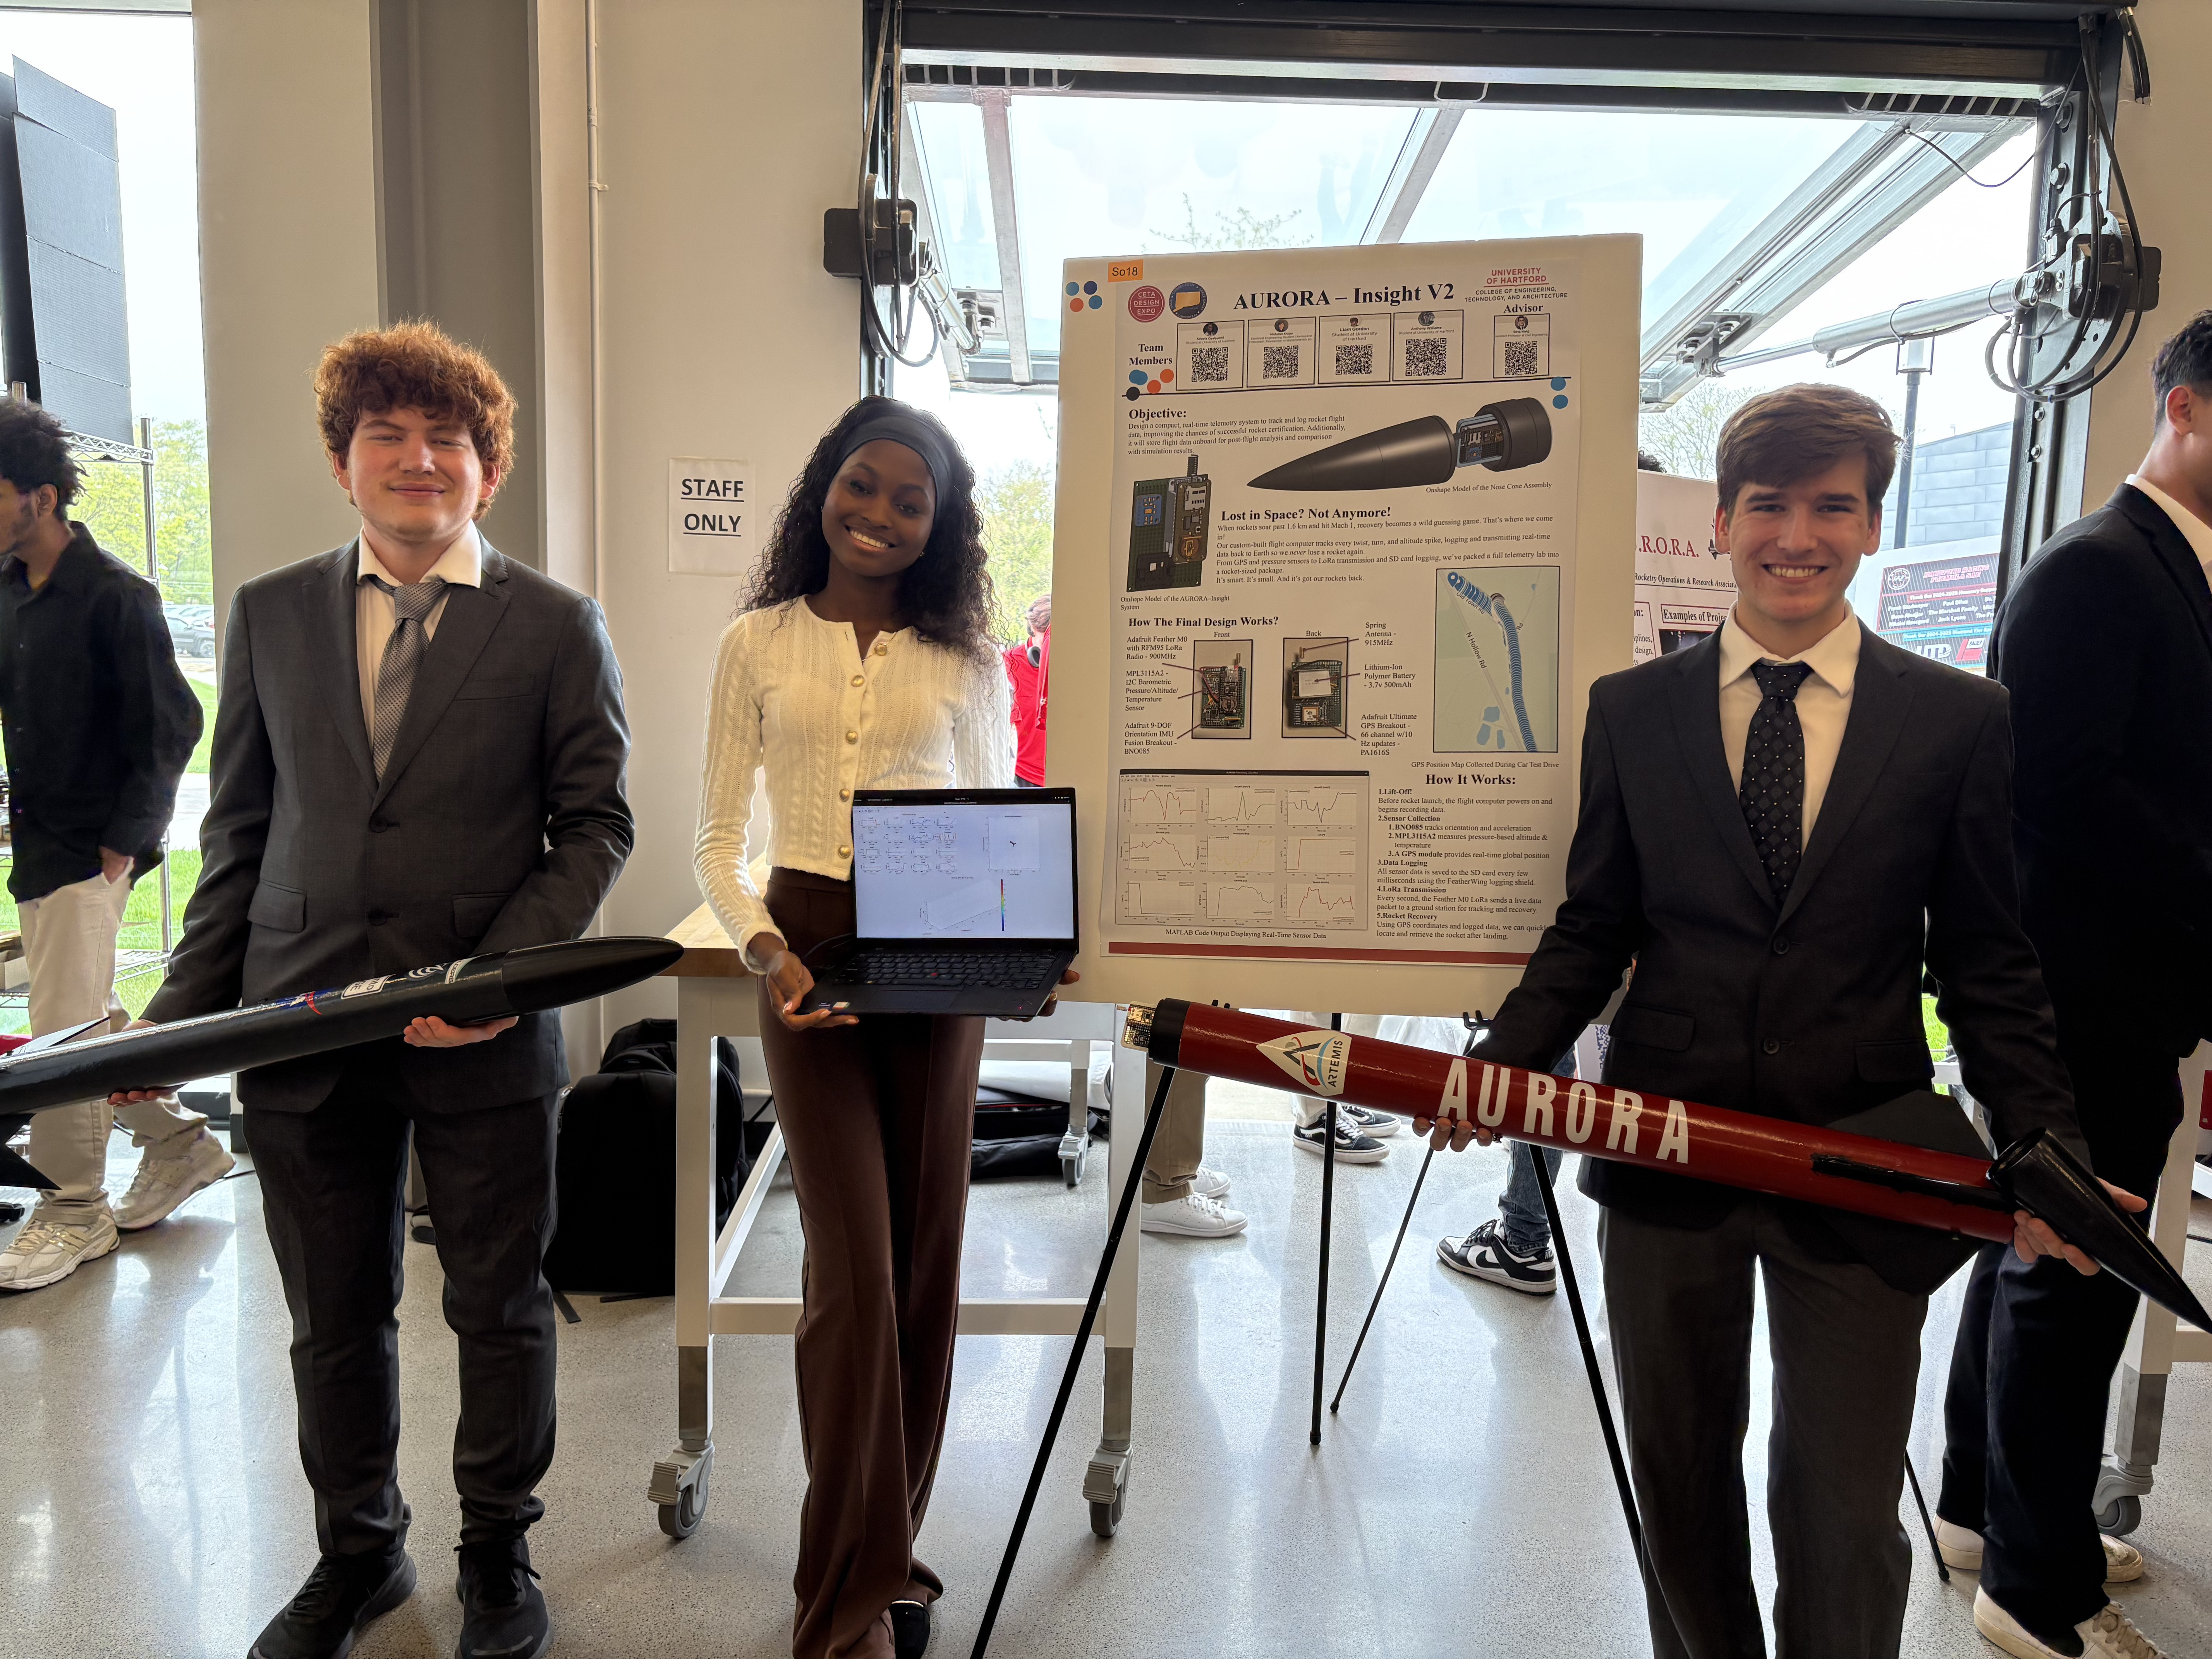
\includegraphics[width=\columnwidth]{SophomoreExpo.jpg}
    \caption{AURORA members Nicholas Krupa, Liam Gordon, and Adeola Oyebunmi presenting an early generation of the AURORA Insight Module at the University of Hartford Engineering Expo. The project established early flight-sensing and telemetry concepts that later evolved into the current \deimos{} subsystem.}
    \label{fig:sophomore_expo}
\end{figure}

A subsequent telemetry configuration was successfully flown aboard a Level 1 certification rocket and transmitted vehicle data through a \SI{915}{\mega\hertz} radio link. Experience from these early systems demonstrated the usefulness of real-time telemetry for both flight analysis and vehicle recovery while identifying limitations associated with size, wiring complexity, modular development hardware, and communication performance. The AURORA Insight V3 hardware and associated ground station are shown in Fig.~\ref{fig:insight_v3}.

\begin{figure}[htbp]
    \centering
    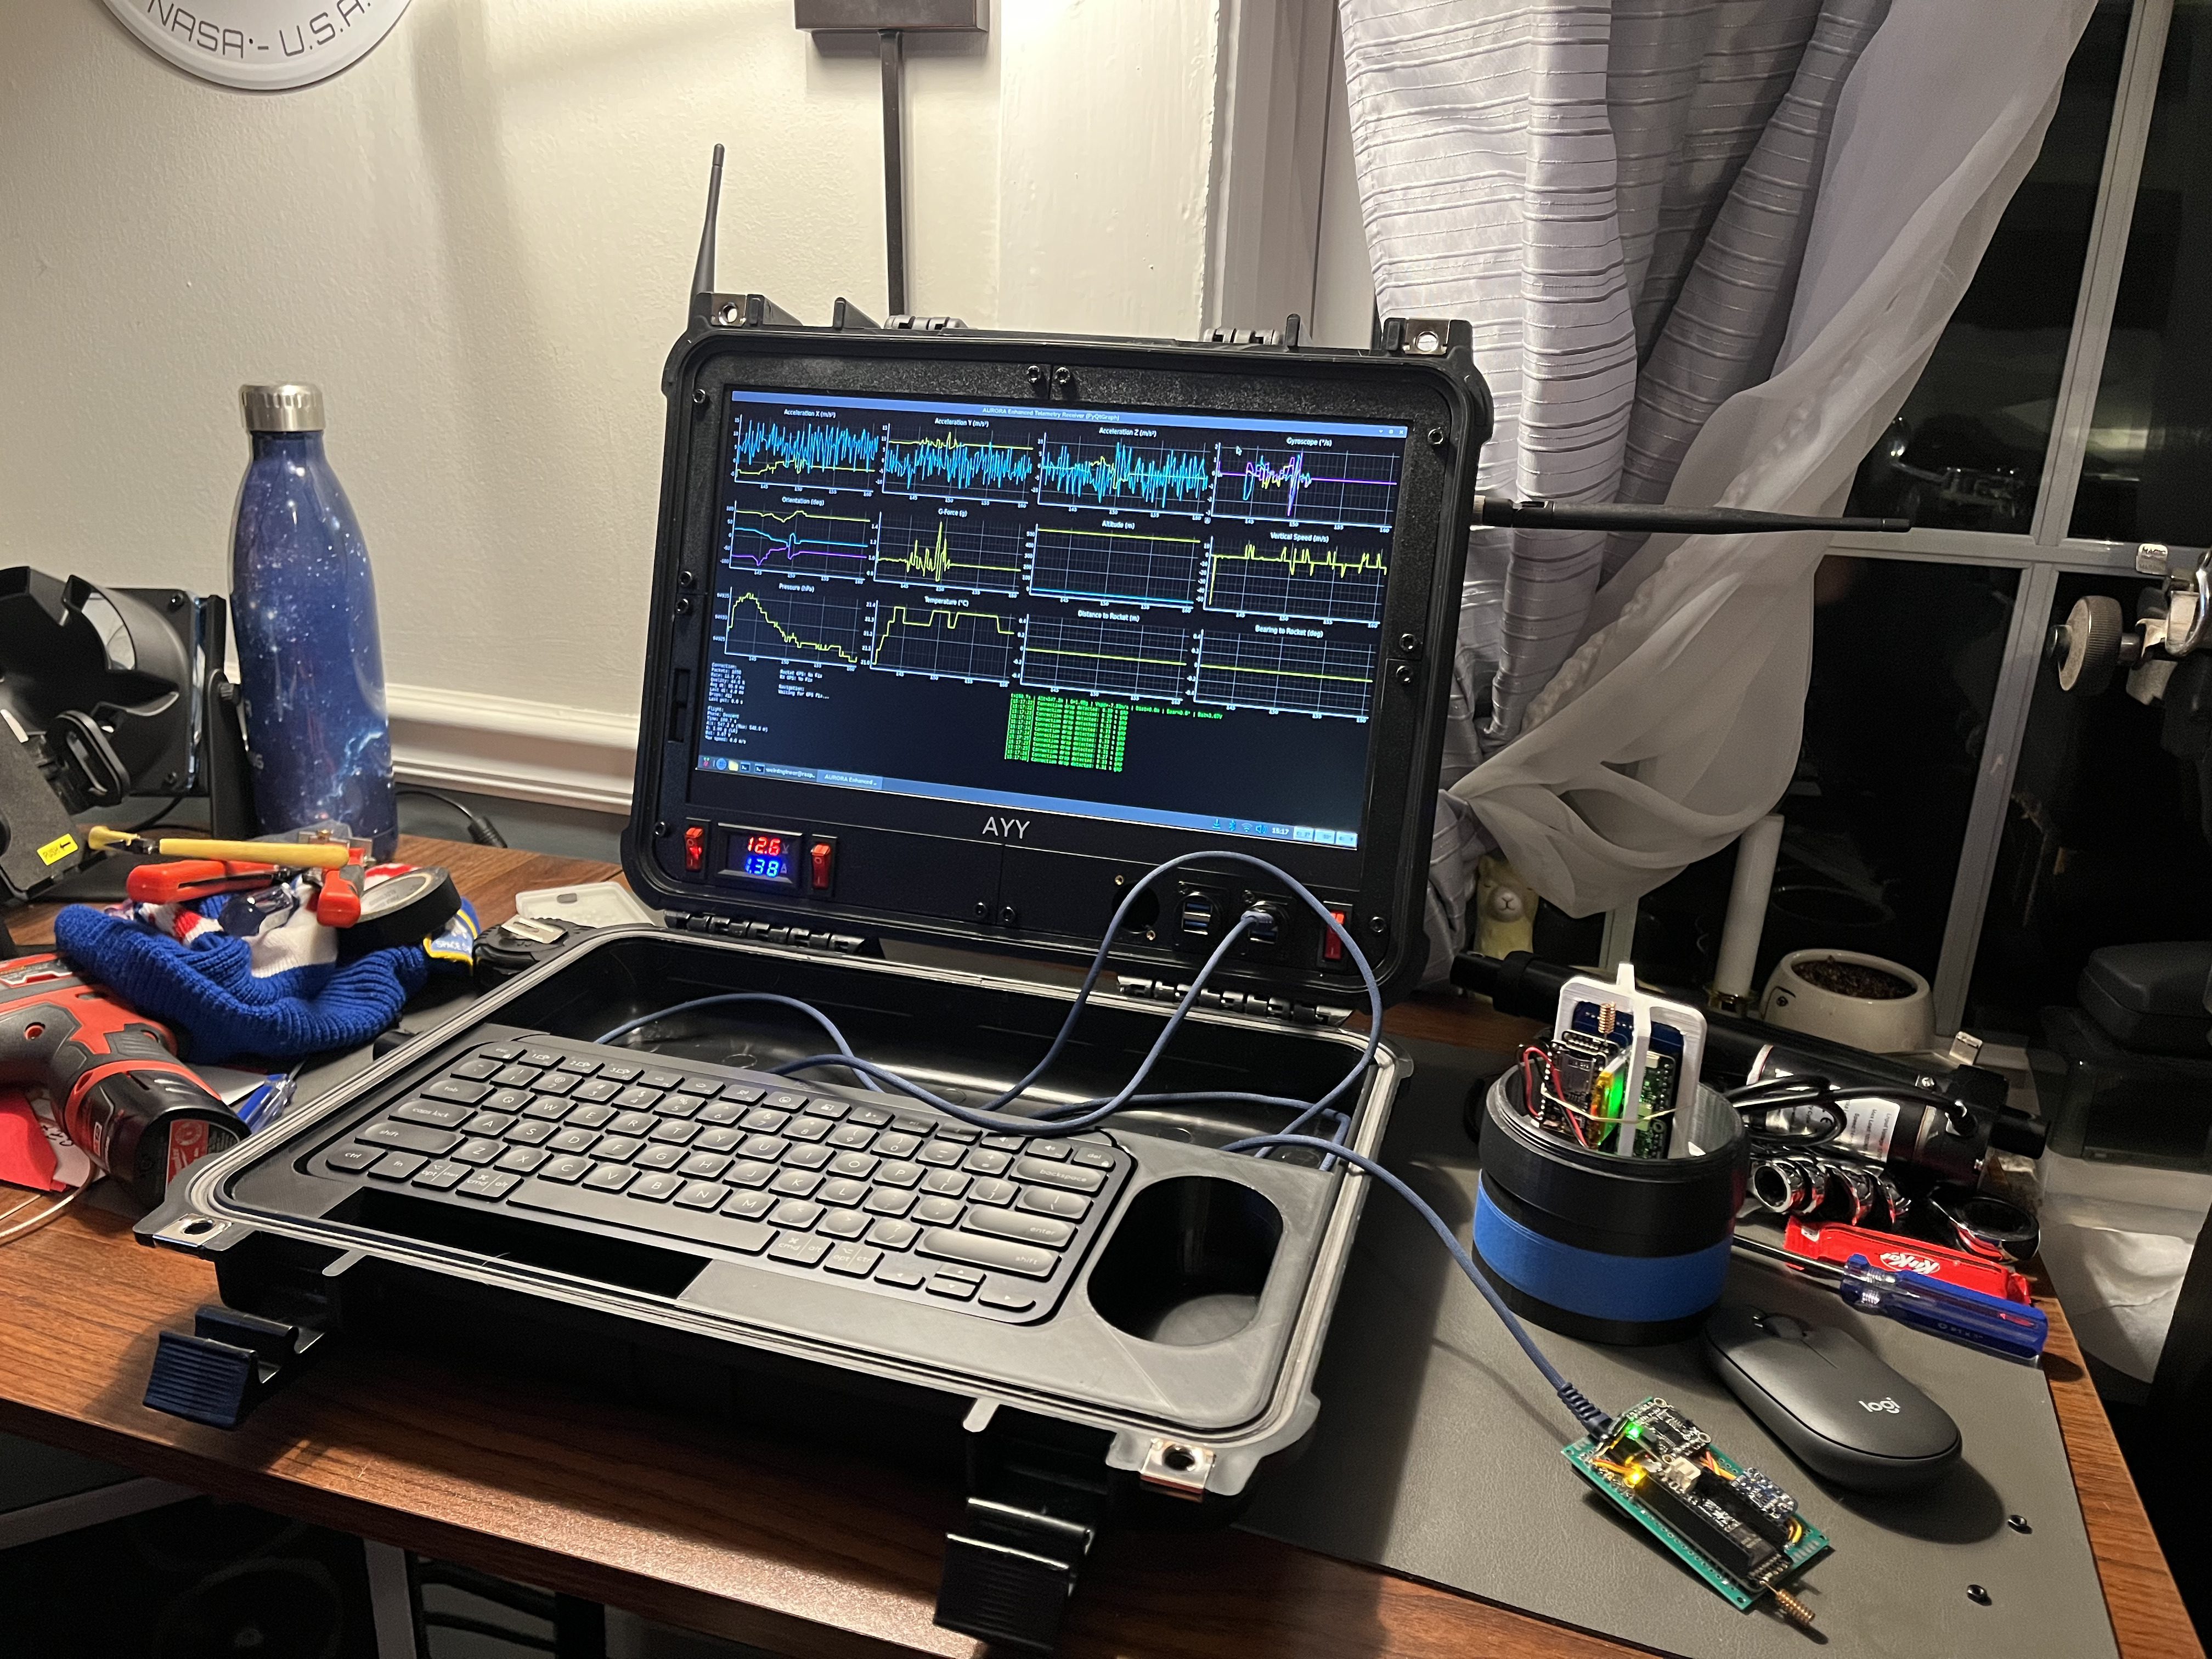
\includegraphics[width=\columnwidth]{InsightV3GroundStation.jpg}
    \caption{AURORA ground station alongside the third-generation AURORA Insight telemetry system. The modular arrangement used commercially available development hardware and external interconnects; experience with this configuration motivated the more compact, fully embedded sixth-generation \deimos{} architecture.}
    \label{fig:insight_v3}
\end{figure}

The sixth-generation design will focus on improving reliability, compactness, telemetry range, and achievable data rate. Previous generations relied heavily on interconnected commercial development boards and external modules. The new system will instead be developed around a fully custom printed circuit board containing the primary processing, sensing, data logging, power-management, and communication hardware required by the subsystem.

Development of this revision includes schematic design, circuit simulation, component selection, PCB layout, fabrication, assembly, embedded software development, and hardware validation. This represents a significant expansion from earlier prototype-based systems because the complete avionics architecture must now be designed and integrated at the board level.

Particular attention will be placed on power integrity, signal integrity, sensor interfacing, connector reduction, mechanical integration, and the ability of the electronics to remain reliable under high-power rocket flight conditions. Reducing the number of independently connected modules and wiring interfaces is expected to improve both packaging efficiency and system reliability.

The communication architecture also represents the project's first substantial transition into RF hardware design. Rather than treating the radio only as an externally connected commercial module, the development process will consider RF signal routing, transmission hardware, impedance-controlled PCB layout, antenna interfaces, grounding, signal integrity, and overall communication-link performance.

Through this redesign, \deimos{} will serve as the primary real-time telemetry and flight-data platform for \ares{} while demonstrating a fully embedded student-designed avionics system. The platform is also intended to establish a foundation for future AURORA developments involving higher-performance telemetry, RF electronics, navigation, and integrated flight instrumentation.

At the time of writing, development of the sixth-generation \deimos{} hardware is included within the scope of prospective sponsorship discussions with Ensign-Bickford Aerospace \& Defense (EBAD). Potential support would contribute toward PCB fabrication and assembly, avionics hardware, RF hardware, system integration, and validation testing.

% =========================================================
\section{Conclusion}

The \ares{} capstone project combines several independently developed engineering systems into a unified high-power research vehicle. The vehicle itself provides the structural, aerodynamic, propulsion, recovery, and integration platform required to support the mission. \phobos{} introduces experimental phased-array and RF research, \comet{} provides student-developed flight-critical recovery control, and \deimos{} advances several generations of AURORA telemetry development toward a fully embedded avionics architecture.

Together, these systems provide a multidisciplinary capstone effort spanning mechanical engineering, electrical engineering, embedded systems, RF engineering, simulation, manufacturing, testing, and flight operations. Beyond the primary mission, the project is intended to establish a reusable research platform and technical foundation that can support continued undergraduate aerospace development at the University of Hartford.